\documentclass[11pt,a4paper]{article}
\usepackage[utf8]{inputenc}
\usepackage[T1]{fontenc}
\usepackage{lmodern}
\usepackage[margin=2.5cm]{geometry}
\usepackage{amsmath,amssymb}
\usepackage{booktabs}
\usepackage{graphicx}
\usepackage{xcolor}
\usepackage{url}
\usepackage[colorlinks=true,linkcolor=blue!50!black,citecolor=blue!50!black,urlcolor=blue!50!black]{hyperref}

\newcommand{\R}{\mathbb{R}}

\title{A topological proxy for the ill-conditioning of the discrete inverse conductance problem,\\ and an independent integrator check of a resistor--capacitor bench}
\author{Xavier Callens\\[2pt]
\small SocrateAI Lab, Cagnes-sur-Mer, France\\
\small \texttt{callensxavier@gmail.com}}
\date{October 2026 \\ \small Preprint, not peer reviewed. Companions: doi:10.5281/zenodo.23228685 and doi:10.5281/zenodo.23241463}

\begin{document}
\maketitle

\begin{abstract}
The Jacobian of the Dirichlet-to-Neumann map of a resistor network with respect to its edge conductances has one column per edge, and the exponential growth of its condition number with the
depth of the unknowns is the central finding of the companion preprints. Here we ask what persistent homology (GUDHI, Vietoris--Rips, $H_0$) sees in the cloud of these columns, layer by layer in depth.
On a square disk the median $H_0$ death time of a layer, which is the typical angle between neighbouring columns, falls with depth like one over the depth (a power law, found after the data), while the smallest singular
value falls exponentially; the two are strongly correlated across layers because both are monotone, but the topological proxy does not give the rate. On the $\{7,3\}$ tiling the proxy shows no collapse over the four layers available,
consistent with the polynomial growth of the condition number there. The preregistered exponential size of the effect was wrong, and two known-answer gates failed as written through design errors of mine, which are kept. In a second, independent
experiment, the rusty-SUNDIALS CVODE integrator reproduces the exact modal step responses of the proposed garage board to within $2\times10^{-6}$ of the supply voltage and the fitted time constants to $3\times10^{-5}$, and the predicted ratio of time constants of the
hyperbolic and the square board, $0.604\pm0.03$, survives a 1\,\% component spread with a scatter of about 1\,\%. Neither result concerns holography or any hardware measurement.
\end{abstract}

\section{Introduction}
Exponential ill-conditioning of the inverse conductivity problem and of its discrete versions is classical~\cite{DiCristoRondi,BorceaReview}. The companion preprints~\cite{Preprint,StripPaper} measured it for the Jacobian of the Dirichlet-to-Neumann (DtN) map of resistor networks,
found it exponential in the depth of the unknowns on flat lattice disks and polynomial on hyperbolic tilings, and gave an exact rate on a solvable strip. Earlier topological work in this programme applied persistent homology~\cite{ELZ} to the boundary resistance metric to detect bulk defects,
and found that deep defects leave no topological signature. This note turns the tool on the object that carries the conditioning result: the columns of the Jacobian. If ill-conditioning means that the columns of deep edges are nearly parallel to others,
a Vietoris--Rips filtration of the column cloud should show it. The second part is unrelated in method but shares the purpose of the programme: the garage experiment predicts a time-constant ratio between a hyperbolic and a square resistor--capacitor board, and the code that
produces the predicted step responses solves the network exactly by an eigendecomposition. We check it against a different method, the stiff integrator CVODE of SUNDIALS~\cite{SUNDIALS} used through the Rust port rusty-SUNDIALS.

\section{The column cloud}\label{sec:cloud}
The Jacobian column of edge $e=(a,b)$ is $J_e=\mathrm{upper}(d_ed_e^{\top})$ with $d_e$ the difference of the rows of the harmonic extension at $a$ and $b$, upper meaning the strictly upper triangle. Inner products of columns are
$\langle J_e,J_f\rangle=\tfrac12[(d_e\!\cdot\! d_f)^2-\sum_i d_{e,i}^2d_{f,i}^2]$, so no $J$ is formed. The distance between edges is the sine of the angle between the lines, $\delta=\sqrt{1-c^2}$ with $c$ the cosine. The depth of an edge is the smaller graph distance
of its endpoints to the boundary. For each depth layer we compute the Vietoris--Rips filtration~\cite{GUDHI} on $\delta$ and read the $H_0$ death times, which are the edge weights of the minimum spanning tree (checked against an independent computation in every layer).
The layer statistic is the median death time $m_k$. Controls: a random cloud of unit Gaussian vectors in the same ambient dimension with the same layer sizes; a cloud of exactly duplicated columns.

\paragraph{Preregistered predictions} (preregistration 30, committed before the run): the median death time falls with depth on the square disk (Spearman correlation at most $-0.9$); its slope against depth is smaller in magnitude on the $\{7,3\}$ tiling; its logarithm
correlates with $\log_{10}\sigma_{\min}$ of the restricted Jacobian (at least $0.9$); and the slope on the square disk lies between $-1.5$ and $-0.3$ decades per layer (a band chosen without a pilot).

\paragraph{Results.} Table~\ref{tab:cloud} and Figure~\ref{fig:cloud}. The first three predictions held. The fourth was refuted: the slope is $-0.078$ per layer, an order of magnitude below the band. The post hoc form is a power law: $k\,m_k$ is between $2.2$ and $2.3$ for layers $3$ to $9$,
the log--log slope is $-0.96$, and the root-mean-square residual is $0.008$ against $0.061$ for an exponential. The random control is flat (slope $5\times10^{-6}$). On the $\{7,3\}$ tiling the median death times stay between $0.87$ and $1.00$ over the four layers (slope $+0.016$).
The correlation with $\log\sigma_{\min}$ ($0.994$) is real but is that of two monotone sequences.

% GENERATED by make_paper2.py from data/*.json -- do not edit
\begin{table}[t]\centering\small
\caption{Square disk of radius 16: edges per layer, median $H_0$ death time $m_k$ of the sine-distance cloud of Jacobian columns, $k\,m_k$, and $\log_{10}\sigma_{\min}$ of the Jacobian restricted to depth $\le k$. On the $\{7,3\}$ tiling (5 layers) the median death times are 1: 0.869, 2: 0.997, 3: 0.966, 4: 0.990.}
\label{tab:cloud}
\begin{tabular}{ccccc}\toprule
$k$ & edges & $m_k$ & $k\,m_k$ & $\log_{10}\sigma_{\min}$ \\ \midrule
2 & 148 & 0.876 & 1.752 & -4.842 \\
3 & 140 & 0.746 & 2.238 & -6.179 \\
4 & 132 & 0.551 & 2.204 & -7.406 \\
5 & 124 & 0.453 & 2.263 & -9.260 \\
6 & 108 & 0.377 & 2.259 & -10.154 \\
7 & 100 & 0.324 & 2.266 & -10.991 \\
8 & 92 & 0.287 & 2.299 & -12.402 \\
9 & 76 & 0.258 & 2.322 & -13.242 \\
\bottomrule\end{tabular}\end{table}

\begin{table}[t]\centering\small
\caption{Integrator check: for each of six draws per board (5\,\% resistors, 10\,\% capacitors), the CVODE tolerances used, the maximum difference to the bench's modal solution in units of $V_0$, and the relative difference of the fitted time constant. Ratio of fitted time constants $\{7,3\}$/square over 12 draws at 1\,\%: mean 0.605, range 0.600--0.608, spread 0.013.}
\label{tab:cvode}
\begin{tabular}{llcc}\toprule
Board & (rtol, atol) & max $|\Delta V|/V_0$ & $|\Delta\tau|/\tau$ \\ \midrule
{7,3} L=2 & (1e-10, 1e-10) & 5.4e-08 & 6.6e-07 \\
{7,3} L=2 & (1e-10, 1e-10) & 6.1e-08 & 6.5e-07 \\
{7,3} L=2 & (1e-10, 1e-10) & 5.4e-08 & 6.1e-07 \\
{7,3} L=2 & (1e-10, 1e-10) & 5.6e-08 & 6.5e-07 \\
{7,3} L=2 & (1e-10, 1e-10) & 5.1e-08 & 5.4e-07 \\
{7,3} L=2 & (1e-10, 1e-10) & 5.4e-08 & 6.0e-07 \\
square R=6 & (1e-08, 1e-08) & 1.8e-06 & 3.0e-05 \\
square R=6 & (1e-08, 1e-08) & 1.8e-06 & 3.1e-05 \\
square R=6 & (1e-08, 1e-08) & 1.7e-06 & 2.8e-05 \\
square R=6 & (1e-08, 1e-08) & 1.7e-06 & 2.8e-05 \\
square R=6 & (1e-08, 1e-08) & 1.7e-06 & 3.0e-05 \\
square R=6 & (1e-08, 1e-08) & 1.8e-06 & 3.1e-05 \\
\bottomrule\end{tabular}\end{table}

\begin{table}[t]\centering\small
\caption{Register of the preregistered gates and predictions, from the stored verdicts. Every refutation and failed gate is kept.}
\label{tab:register2}
\begin{tabular}{llp{6cm}}\toprule
Prereg. & Item & Verdict \\ \midrule
30 & G1 control & pass \\
30 & G2 duplicated columns & fail (limit unattainable, Sec.~\ref{sec:fail}) \\
30 & G3 clipping & pass \\
30 & P1 collapse (square) & held \\
30 & P2 flat vs hyperbolic & held \\
30 & P3 tracks $\sigma_{\min}$ & held \\
30 & P4 exponential size & refuted \\
31 & G1 integrator vs bench & pass \\
31 & P1 waveforms & refuted \\
31 & P2 fitted $\tau$ & held \\
31 & P3 ratio band & held \\
\bottomrule\end{tabular}\end{table}


\begin{figure}[t]\centering
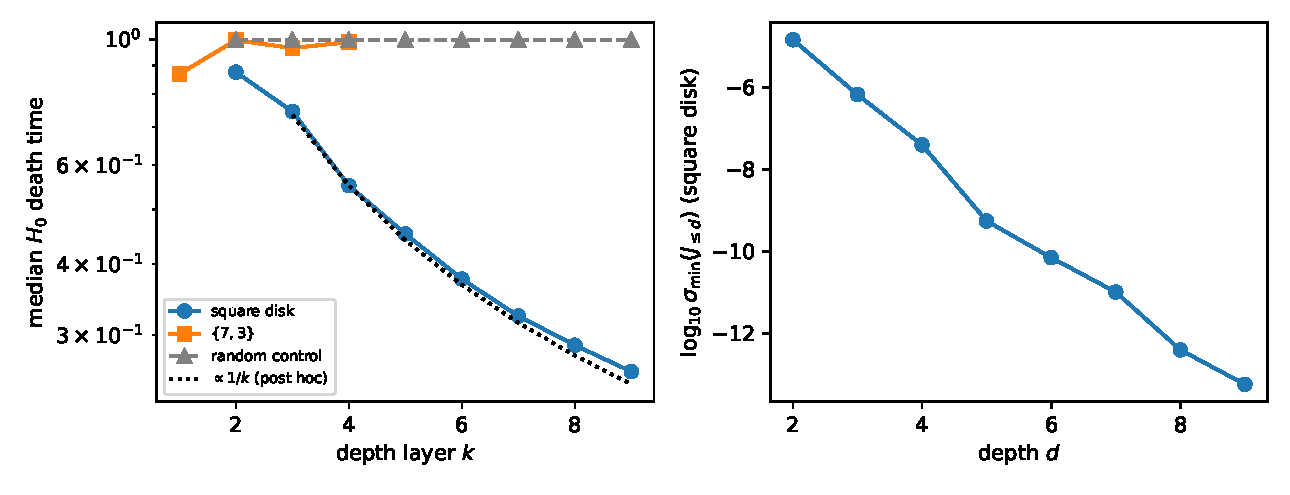
\includegraphics[width=0.95\linewidth]{fig_p2_cloud.pdf}
\caption{Left: median $H_0$ death time of the Jacobian column cloud against depth layer, square disk, $\{7,3\}$ tiling, and a random control; the dotted line is $2.3/k$ fitted after the data. Right: $\log_{10}\sigma_{\min}$ of the restricted Jacobian on the square disk.}
\label{fig:cloud}
\end{figure}

\paragraph{Reading.} Single-linkage $H_0$ sees that deep columns crowd together, and it does so through nearest-neighbour angles, which close slowly (like $1/k$), while the smallest singular value closes exponentially. Ill-conditioning is therefore a property of linear dependence among many columns, which
nearest-neighbour topology cannot resolve. The proxy separates the flat from the hyperbolic case qualitatively, with only four hyperbolic layers. Higher-dimensional persistence ($H_1$ was computed for diagnostics and not scored) and a filtration by principal angles to the span of shallower columns are the natural next steps.

\section{An independent integrator for the garage bench}\label{sec:cvode}
The virtual bench of the lab protocol draws resistors and capacitors with tolerances, ties all boundary nodes to a stepped rail, and evaluates the interior response by the generalised eigenproblem $L_{ii}u=\lambda Cu$. Any error in that code would bias the predicted time-constant ratio.
Preregistration 31 integrates the same perturbed boards with CVODE (BDF) and compares waveforms at three probes (depth classes 1 to 3) and the fitted time constants (the protocol's weighted log-linear fit on $y/V_0\in[0.01,0.10]$).

\paragraph{Results} (Table~\ref{tab:cvode}). The known-answer gate passed after its threshold was relaxed from $10^{-8}$ to $10^{-7}$ of $V_0$ (the binding rejects absolute tolerances below $10^{-10}$ at the first step and the achievable error is set by the absolute tolerance). The fitted time constants agree to $3\times10^{-5}$ (prediction held),
the ratio prediction held, and the waveform prediction (agreement to $10^{-6}$ of $V_0$) was refuted on the square board only, where the integrator had to run at looser tolerances (differences near $1.7\times10^{-6}$), at the level of the integrator's own error; the hyperbolic draws agree to $6\times10^{-8}$.
The check validates the model code, not the hardware: source resistance, probe loading, leakage and parasitics are in neither side.

\section{What failed}\label{sec:fail}
\begin{itemize}
\item The exponential band for the slope of the median death time (prediction P4 of preregistration 30) was set without a pilot and was wrong in kind: the decay is a power law.
\item The known-answer gate on duplicated columns failed twice as written. First, GUDHI drops pairs of zero persistence by default, so exact duplicates never appeared; the rerun reads all pairs and checks them against the minimum spanning tree (the main numbers did not change). Second, the sine distance has a rounding floor near $1.5\times10^{-8}$ for identical columns, so the limit $10^{-12}$ was unattainable; the test is met at that floor, a post hoc reading.
\item The integrator needed three recorded deviations before any scored comparison: time scaled by the nominal time constant, tolerances no tighter than $10^{-10}$ (with the threshold of the known-answer gate relaxed after a debug run showed $1.1\times10^{-8}$), and a ladder of tolerances per draw because the stiffer square board aborts at the tightest setting.
\item In the transient-data experiment of the companion~\cite{StripPaper} a time-to-frequency gate failed through an integration window that ignored the steady current; that is reported there.
\end{itemize}
Gates and predictions are listed in Table~\ref{tab:register2}.

\section{Limits}
The topological result is for one square disk of radius 16 and four hyperbolic layers, in double precision, noise-free, $H_0$ only. The power law is a post hoc description of eight points. The integrator check uses the same model on both sides, with 12 ratio draws and uniform tolerances.
Nothing here concerns holography, AdS/CFT or the physical hardware.

\section*{Reproducibility}
Scripts \texttt{exp30} and \texttt{exp31}, preregistrations 30 and 31, the data under \texttt{data/} and the generator \texttt{paper/make\_paper2.py} are in the repository of the companion preprint. Every table and figure is generated from the stored data. These runs were recorded by the orchestrating model directly and are not entered in the evidence ledger.

\section*{Use of AI tools}
Code, numerical experiments and drafting were carried out with the assistance of Claude (Anthropic). The author directed the work and takes responsibility for the content.

\begin{thebibliography}{99}
\bibitem{Preprint} X.~Callens, Logarithmic boundary depth and the conditioning of the discrete inverse conductance problem on hyperbolic lattices (version 1.2), Zenodo, doi:10.5281/zenodo.23228685.
\bibitem{StripPaper} X.~Callens, Exact exponential rates for the discrete Calder\'on problem on lattice strips, and what transient data do not change, Zenodo, doi:10.5281/zenodo.23241463.
\bibitem{DiCristoRondi} M.~Di Cristo and L.~Rondi, Examples of exponential instability for elliptic inverse problems, arXiv:math/0303126 (2003).
\bibitem{BorceaReview} L.~Borcea, V.~Druskin, F.~Guevara Vasquez and A.~V.~Mamonov, Resistor network approaches to electrical impedance tomography, in \emph{Inside Out II}, MSRI Publications 60 (2012); arXiv:1107.0343.
\bibitem{ELZ} H.~Edelsbrunner, D.~Letscher and A.~Zomorodian, Topological persistence and simplification, \emph{Discrete Comput.\ Geom.} 28 (2002) 511--533.
\bibitem{GUDHI} The GUDHI Project, GUDHI User and Reference Manual, Inria, \url{https://gudhi.inria.fr}.
\bibitem{SUNDIALS} A.~C.~Hindmarsh et al., SUNDIALS: suite of nonlinear and differential/algebraic equation solvers, \emph{ACM Trans.\ Math.\ Softw.} 31 (2005) 363--396.
\end{thebibliography}
\end{document}
